\documentclass[../main.tex]{subfiles}
\begin{document}
\chapter{Introduction}
    \label{ch:chapter1}
    \captionsetup{labelfont=bf}
    \graphicspath{{Chapter1/}}


%As you type and reference things, you can use \hyperref[label]{DisplayedText} to make a link to a different chapter or section of a chapter. \autoref{label} also works, but then it might not write exactly what you want (e.g., referencing to "Chapter 2").
%I used a mix of types of delineations: 
	%\section[Short title that appears in TOC]{Actual text that apperas in place in the document} 
	%\subsection \subsubsection \paragraph
	% Table of contents only showed down to subsection... subsubsection and paragraph do not appear in the TOC
	%\begin{enumerate} \item \end{enumerate}
	%Occasionally I inserted \footnote but mostly tried to avoid that.

%Include a citation at the beginning of the chapter if it has been previously published in whole or in part.
\section{Protein conformational landscapes encode functional information.}
	Proteins are the machines that power cellular function and life. They allow us to see, smell, think, and carry out many of the basic functions required for us to live. However, when they malfunction or misbehave (usually through mutation), they can also result in diseases like cancer or heart disease among others. Proteins are also utilized by viruses and bacteria to infect host cells, replicate, or even break down the drugs we use to stop them.

	Understanding protein behaviors relevant to health and disease depends on being able to model them in atomic detail. Atomistic scale motions allows us to infer things like mechanisms, thermodynamic profiles, and kinetic rates. This level of detail can provide predictive models and explanations for why certain mutations may cause disease, which can be useful for targeting proteins using drug design methods. Furthermore, knowledge of chemical interactions allows us to design chemical groups against pockets that would jam them open\cite{Roth:2017gk}. Atomic-scale knowledge may even provide guiding principles upon which proteins can be designed to perform novel functions, which has implications for therapeutic design and industrial applications\cite{weitzner_computational_2019}.

	Structural biology methods have been transformative in allowing us to learn about the structure of proteins and their behaviors. The first view of protein structures was done using X-Ray crystallography\cite{kendrew_three-dimensional_1958}. However, static structures do not provide a complete picture of protein function. These static structures may not be able to provide information about a proteins stability \cite{khan_performance_2010}, ligand affinities or specificities\cite{yin_overview_2017}, or how different mutations could impact function\cite{Hart:2016kb}. Indeed, it has been often observed that crystal structures of the same protein families are too similar to explain the difference in their measured physiological parameters\cite{porter_conformational_2020}.

	As the atoms of a protein move around relative to one another, a protein is able to shift between an enormous number of different structures. Even small proteins of $<$100 amino acids have ~$\sim$200 rotatable bonds along their backbone, granting access to more than $10^{60}$ backbone conformations \cite{levinthal_how_1969}. Many of these structures however are never accessed by the protein in physiologically relevant timescales.  Of the fraction that are accessed however, some of them may have relevance to a protein’s mechanism and biophysical behavior. Each of these structures that a protein may shape-shift into has an associated energy that characterizes intra-protein and protein-environment interactions. Given that the probability of a protein adopting any one structure is proportional to the exponential of that structures energy, we are able to characterize how likely a protein is to adopt some states over others. The phase space of a protein’s energies (or probabilities) and their corresponding structures are often referred to as an “energy landscape”, with most likely states (such as those observed by crystallography) are named “ground” states due to being energy minima. 

	 From these ground states, a protein can also transition into less likely “excited” states, some of which may contain key functional information. These states can be characterized using a plethora of methods. Nuclear Magnetic Resonance (NMR) and Hydrogen-Deuterium Exchange (HDX) have provided unique functional insight into the conformational heterogeneity a protein can have\cite{baldwin_early_2011,HenzlerWildman:2007cz}. Work on DHFR has been critical in understanding the complete catalytic cycle and the residue level configurations (and dynamics)\cite{Boehr:2006jd}. NMR experiments on DHFR that was arrested in one stage of its catalytic cycle provided evidence that DHFR was also adopting stages in the latter part of its cycle\cite{Boehr:2006jd}. Mutational experiments also put forth a correlation between dynamics and catalytic ability\cite{Boehr:2006jd,Boehr:2009ju,HenzlerWildman:2007cz}. Powerful combinations of NMR, crystallography, and computer simulations have rationalized cofactor- and mutational-effects on kinases\cite{zorba_molecular_2014,kerns_energy_2015}. With advances in structural methods, it is even possible to resolve structural information about excited states\cite{Boehr:2006jd,Boehr:2009ju}. Other electron paramagnetic resonance (EPR) experiments have granted unique insight into the conformational distributions of proteins\cite{VanEps:2010by}. NMR also has the additional power to measure the degree of conformational entropy of residues\cite{Wand:2013dz}. Recently, Cryo-EM structures of even large complexes have revealed the degree of conformational heterogeneity in physiologically relevant systems\cite{Koehl:2018fv,DraperJoyce:2018il,GarciaNafria:2018hu,Kang:2018kq}. However, it is important to note that each of these methods have tradeoffs due to resolution limits, labelling strategies that may perturb the system, or technical limitations (system size, material requirements, etc.). Altogether, this large body of work studying excited states of folded proteins suggests that the equilibrium motions of a protein may encode all of its functionally relevant states. 

	Molecular dynamics (MD) simulations have the potential to provide atomistic detail to explain complex biological processes. These simulations compute the movements of atoms over time by integrating Newton’s laws of motion over each atom. Thus, MD acts as a “computational microscope”, allowing us to observe the different conformations a protein adopts\cite{Dror:2012cs,lee_discovery_2009}. A perfect simulation would completely describe a protein’s thermodynamic and kinetic behaviors at equilibrium. However, there are major limitations: ($i$) The accuracy of atomic parameters (aka "force fields") that are used to describe atomic interaction (A topic that is discussed extensively elsewhere\cite{kukol_current_2015}). ($ii$) Simulations take femtosecond-sized timesteps, making it expensive to gather data at biologically relevant timescales (microsecond to milliseconds). ($iii$) Interpreting large datasets with thousands of unique structures to generate biologically meaningful predictions remains a daunting task.

\section{The Folding@home platform allows access to protein motions at biologically relevant timescales.}
	\subsection{Folding@home distributes simulations across thousands of computers at once.}
		A myriad of methods have been developed to improve sampling of protein motions out to biologically relevant timescales\cite{E:2010hs,hamelberg_accelerated_2004,paschek_replica_2007,piana_bias-exchange_2007}. However, many perturb the thermodynamics or kinetics of a system, in turn biasing the predictions these simulations make. The advent of GPUs provided access to longer timescales, but they are bounded by an upper limit of parallelism in computing architectures\cite{stone_accelerating_2007,friedrichs_accelerating_2009,eastman_openmm:_2010,eastman_openmm_2017}. Recently, novel adaptive sampling techniques have allowed for the mapping of slower motions\cite{zimmerman_fast_2015} but may require system-specific knowledge or an order parameter of relevance. Specialized hardware has also been developed\cite{shaw_anton_2008} that allowed computational biophysicsts to study processes at unprecedented timescales. However, utilizing and maintaining this kind of specialized hardware can be a costly endeavor. 

		To sample unbiased simulations at biologically relevant timescales using commodity hardware, the Folding@home platform was developed in 2000\cite{Shirts:2000du}. Folding@home, headquartered at the Bowman lab at WUSTL, is a distributed computing network that runs MD simulations on donated computing power thanks to thousands of citizen-scientists who download the app onto their hardware. Folding@home runs trajectories as small “work units” that are smaller simulations on the order of nanoseconds. The starting file for a work-unit is generated server-side, which is sent to a client computer somewhere in the world (Fig. \ref{fig:ch1-fig1}). The client then runs the work-unit and returns it. This is used to generate the subsequent work-unit (representing the next chunk of time in a simulation). Afterwards, work units are stitched together to generate a single trajectory. Folding@home allows for the generation of a datasets containing hundreds of trajectories that, in aggregate, capture a large amount of a protein's energy landscape. These datasets are so large that interpreting them presents a unique “big data” challenge, and requires the development of new methods and software\cite{Husic:2018iz,porter2018enspara}.

        \begin{figure}[!htb] %Positioning code for figure
            \centering
            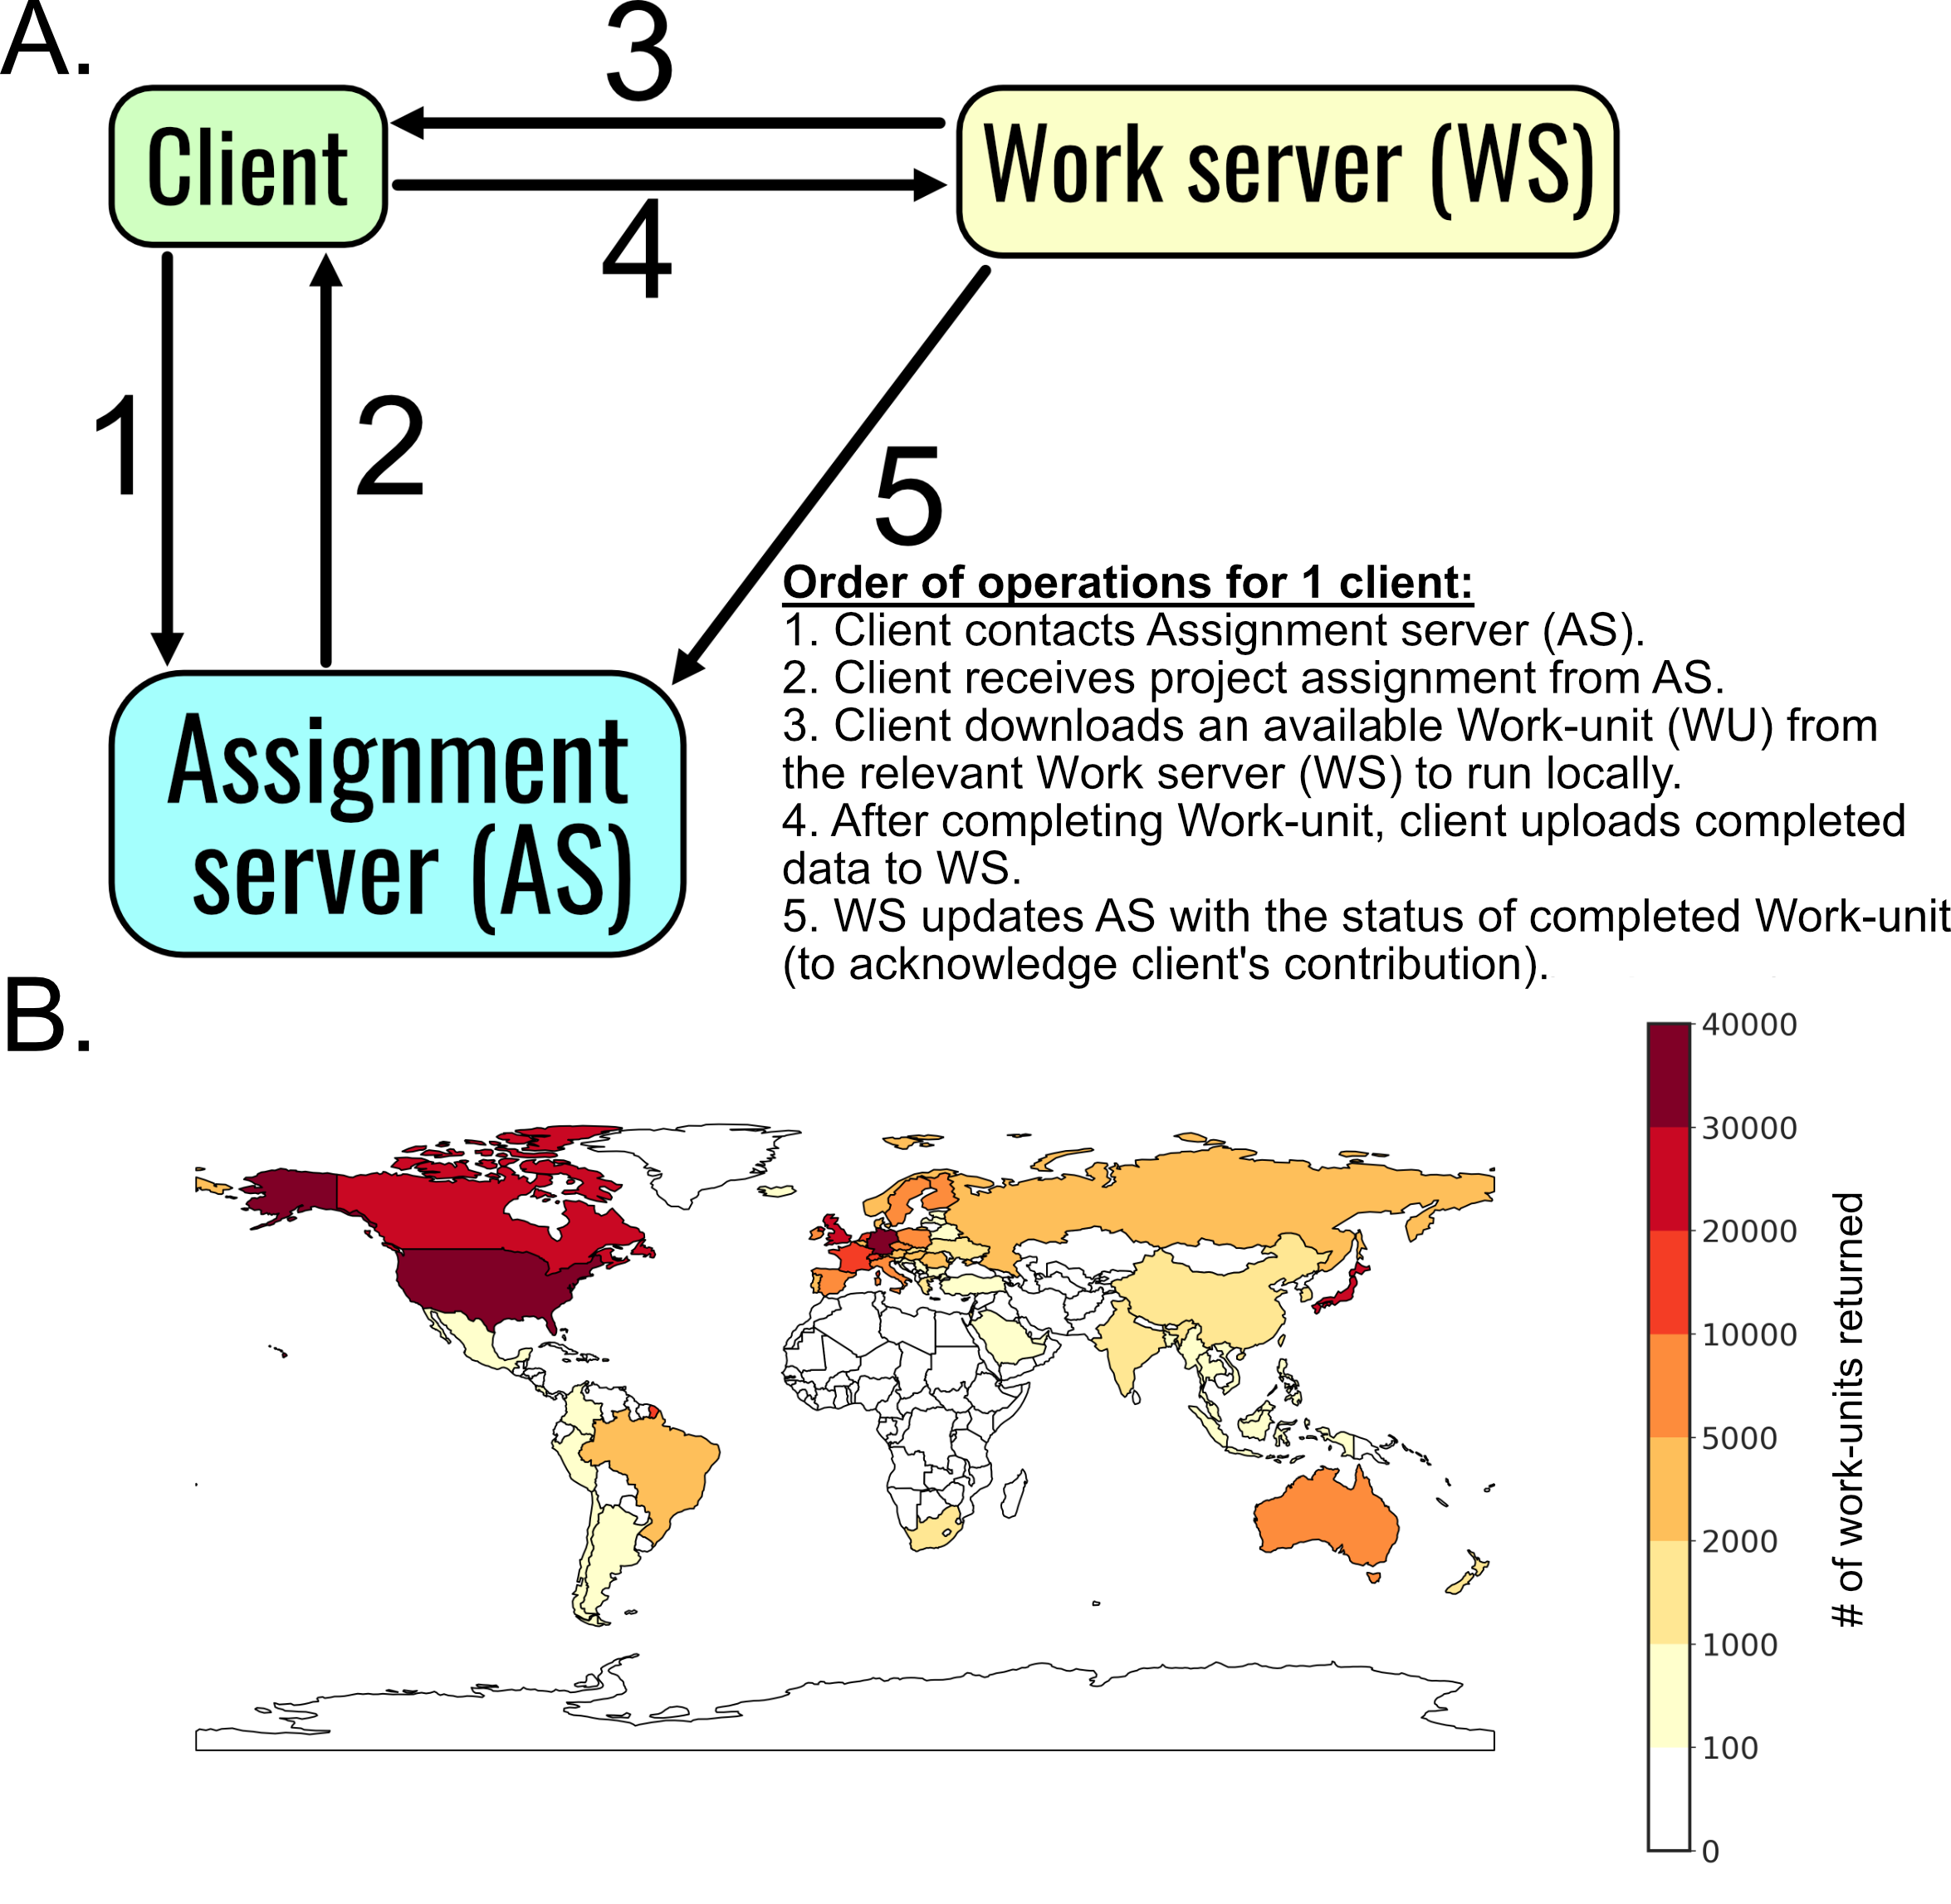
\includegraphics[width=5in]{ch1-fig1.png}
            \caption[Folding@home distributes work units worldwide to run simulations]
                {Folding@home distributes work units worldwide to run simulations \textbf{A.} Workflow schematic detailing the steps a citizen-scientist's computer ("client", green) takes to receive, run, and return a work-unit successfully by communicating with the Assignment Server (blue) and the Work server (yellow). \textbf{B.} Heatmap of completed work-units returned from each country in the world in a representative 48-hour period. The number of returned work units is indicated by the color scale (right).}
            \label{fig:ch1-fig1}
        \end{figure}

	\subsection{Markov State Models allow for the construction of unified models from large simulation datasets.}

		Markov state models (MSMs) are network representations of a protein’s free-energy landscape, providing map representations of protein conformational space with thermodynamic and kinetic properties taken from equilibrium simulations (Fig. \ref{fig:ch1-fig2}). Rather than depending on a single long simulation that explores multiple states sequentially, MSMs are capable of stitching together multiple short trajectories into a single unified landscape. Thus MSMs capture slow events, and their intermediates, far beyond the reach of any individual simulation. Thanks to distributed networks like Folding@home, gathering large numbers of short trajectories is tractable in a reasonable time-frame. Many reviews have been dedicated to providing accessible and in-depth explanations of MSM technology\cite{Chodera:2014gk,Husic:2018iz,Knoverek:2018kk}.

        \begin{figure}[!htb] %Positioning code for figure
            \centering
            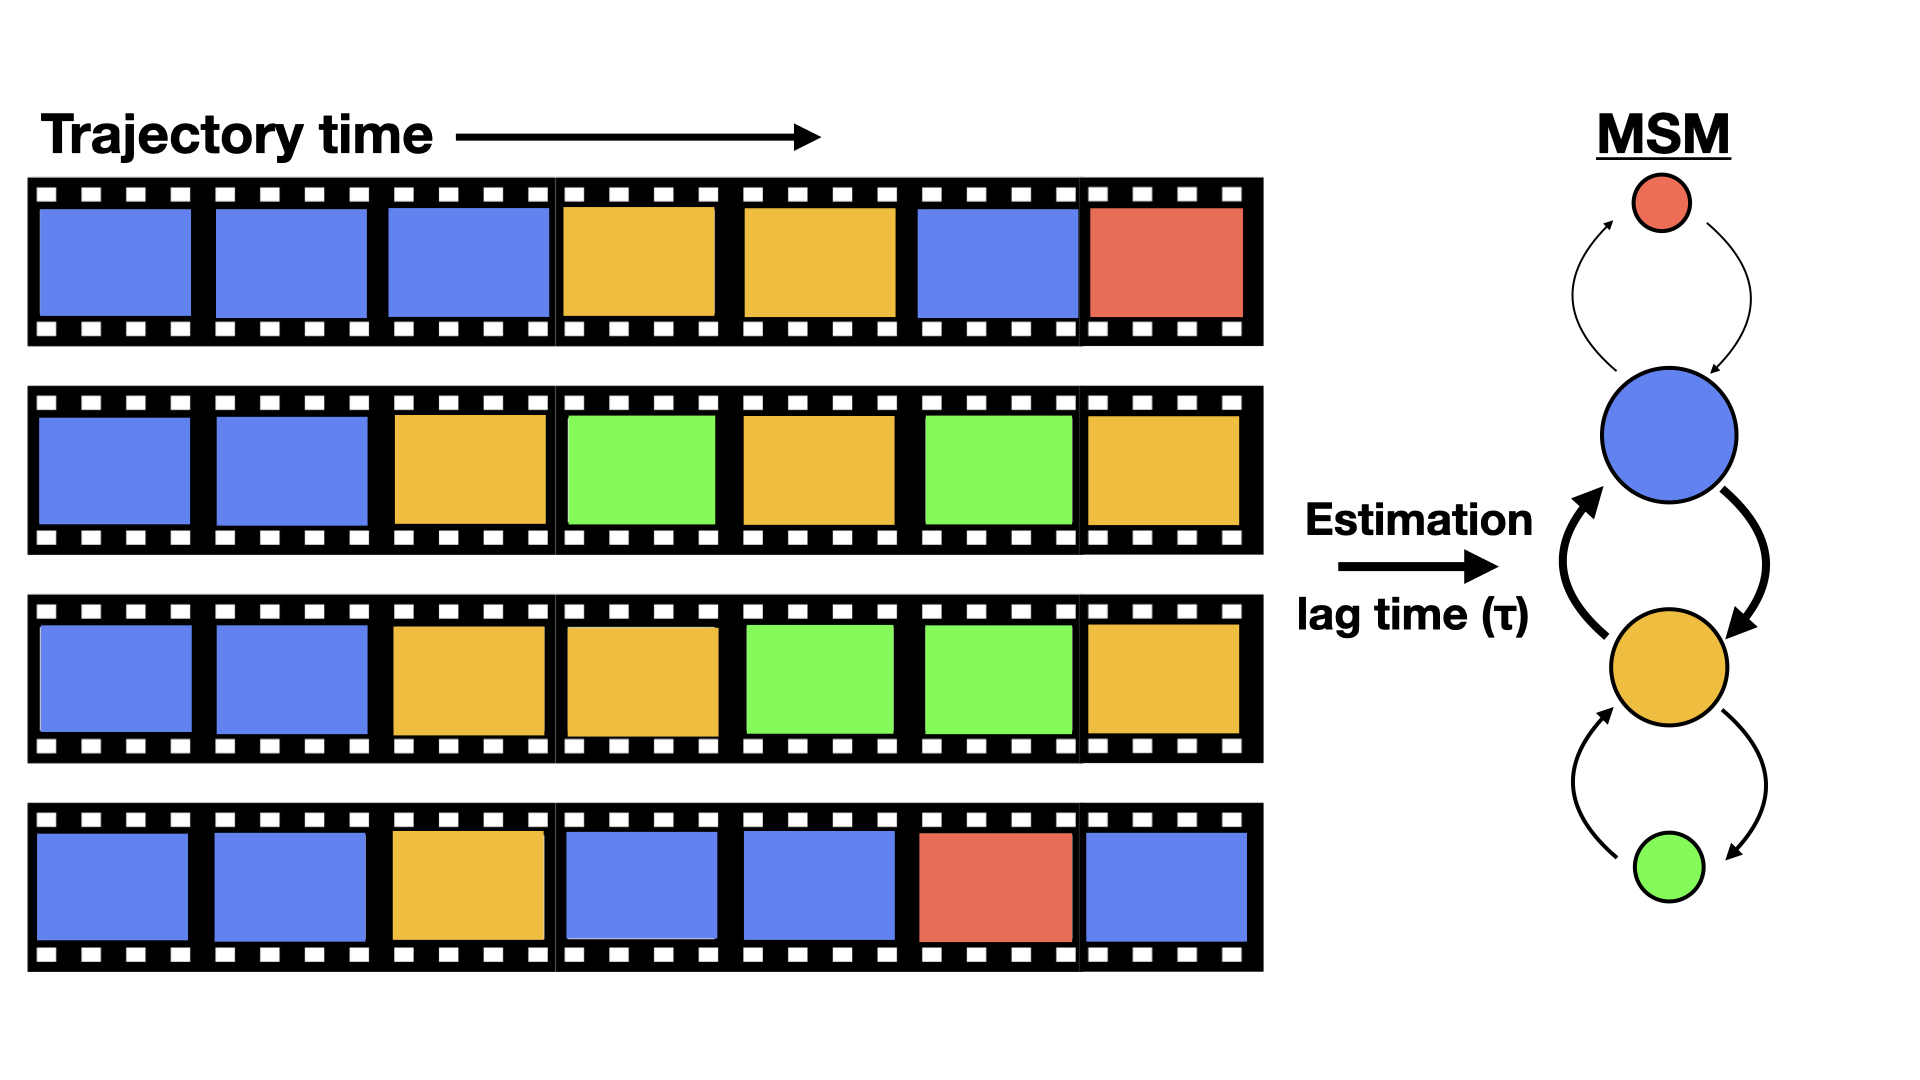
\includegraphics[width=\linewidth]{ch1-fig2.jpeg}
            \caption[Scheme highlighting the conversion of a simulation dataset into a Markov State Model (MSM)]
                {Diagram highlighting the conversion of a simulation dataset into a Markov State Model (MSM). Simulation trajectories (left) are parsed into discrete states on a per-frame basis (red, blue, green, yellow), and estimation methods are used to convert the trajectories into a MSM (right). The spheres radii is proportional to the population of that state, while arrow thickness denotes transition probability.}
            \label{fig:ch1-fig2}
        \end{figure}

		MSMs require two components to describe the dynamics of a biomolecular system: ($i$): A discretization of a high dimensional state space into $n$ conformational states, and ($ii$) A model of the stochastic transitions between each states, represented as a Transition Matrix $\textbf{P}$. The probability of transitioning from state $i$ to state $j$  ($P_{ij}$) is: 

        \begin{equation}\label{transition-matrix-eq}
            % I(X,Y) = -\sum_{x \in X}\sum_{y \in Y} {{\frac{P(x,y)}{P(x)P(y)}}}
            P_{ij}(\tau)=Prob(x_{t+\tau}\in S_j | x_t \in S_i)
        \end{equation} 

        where $\tau$ is a lag-time parameter across which transitions between states are observed, and $S_i$ is state $i$ and $S_j$ refers to state $j$. These transition matrices $\textbf{P}$ give rise to a stationary distribution $\pi$ as a result of the eigenvalue equation: 
        \begin{equation}\label{stationary-dist-eigenvalue-eq}
        	\pi^T\textbf{P}=\pi^T
        \end{equation}
        where $T$ represents a single time-step. In an MSM, the stationary distribution $\pi$ represents the equilibrium probabilities for each state. Therefore, assuming sufficient statistics are collected to observe transitions between states, MSMs are able to appropriately capture the equilibrium thermodynamic and kinetic behaviors of a system. It is important to note that the underlying assumption behind MSM construction is that the discretized dynamics of biomolecules is memoryless (aka Markovian). That is, the probability of a transition from state $i$ to state $j$ at time $t$ is only dependent on state $i$ and not any of the previously visited states.

        For any constructed MSM, the Markovian assumption is tested by looking at implied timescales plots of a Markov State Model. That is, for a given state decomposition, the molecular relaxation timescales for eigenvalues $\lambda$ and eigenvectors $r_i$ are computed for a series of lag-times $\tau$:
        \begin{equation}\label{implied-timescales-eq}
        	t_i=-\frac{\tau}{\ln|\lambda_i(\tau)|}
        \end{equation}
        These timescales $t_i$ are plotted for a series of lag-times $\tau$ (\ref{fig:ch5-suppfig8}). If the timescales remain relatively unchanged for a series of $\tau$ values and higher, then the models constructed for those values of $\tau$ can be considered Markovian. The values of $P_{ij}$ can then be estimated using a variety of estimation methods\cite{Zimmerman:2018jn,Chodera:2014gk}.

        A critical component of high-quality MSM construction is the features selected in the discretization of state space. It is important to balance statistical error against systematic bias when choosing, as narrow features ranges may result in poor statistics, while broadly-ranged features may have large systematic errors due to convolution of multiple motions into a single state. Choice of appropriate feature can challenging due to the sheer size of simulation datasets and the system-specific knowledge often need to identify appropriate features. 

        While methods such as PCA might provide some degree of feature-reduction, a major breakthrough in simulation featurization was the use of time-lagged independent component analysis (tICA)\cite{Molgedey:1994ew}, which transforms input coordinates to identify the rarest (which are assumed to be the slowest) motions. For protein folding simulations, this provides excellent dimensionality reduction, since the slowest coordinate is often the rarest and most valuable \cite{MSultan:2017du,PerezHernandez:2013ih}. However, in simulations of folded proteins the rarest motions observed may be less interesting or artifacts of sampling due to the simulation size. Much success has previously been seen using geometric features, such as cartesian coordinates or dihedral angles\cite{Voelz:2010hs,Bowman:2012jd,Sun:2018kx}. Other features such as solvent accessible surface area (SASA) or ligand-residence-time have also been useful for construction of predictive MSMs \cite{Porter:2019hv,Sun:2018kx}. 

		Once appropriate features are selected, there are a myriad of approaches to cluster them into discrete states. One major method is a hybrid k-centers/k-medoids approach\cite{gonzalez_clustering_1985,park_simple_2009}. In brief, for every pair of features a distance metric, such as the Root Mean Square Deviation (RMSD) is computed. The k-centers algorithm then ($i$) chooses an initial cluster center either as a predetermined point or randomly, and then all points are assigned to this initial cluster. ($ii$) The distance between every point and its assigned cluster center is then computed. ($iii$) The point with the largest distance to the assigned cluster center is then labelled as a new cluster center. ($iv$) The distances between all points and all cluster centers are recalculated, and points are reassigned to their closest cluster center based on these new labels.  Steps ($ii-iv$) are repeated until the maximum distance from any point to its assigned cluster center goes below a specified threshold, or a maximum number of cluster centers is reached.

		To refine the cluster center assignments, and ensure that the “center” of each cluster is truly equidistant from all assigned points, a k-medoids algorithm known as Partitioning around Medoids (PAM)\cite{park_simple_2009} is used. PAM proceeds by iterating through each cluster and choosing a new center from one of the currently assigned points. All points across all states are then reassigned based on this new proposed cluster center. From this proposed center, a "cost" is calculated (i.e. the sum of distances from each point to their respective center), and the proposed center placement is accepted if the cost is minimized. Once states are discretized, clustered, assigned across a simulation trajectory, the transition probability matrix is estimated. As mentioned above, the matrix of transitions between states is counted based on some lag time $\tau$. 

        One simple approach to estimate transitions is to count the number of transitions from states $i$ to $j$ between all states, and divide by the number of states $i$ observed. To maintain ergodicity, some methods only estimate over the largest connected subset of states\cite{prinz_optimal_2011} or using maximum likelihood estimators that respect detailed balance\cite{prinz_markov_2011}. One method to estimate transition probabilities is to to average the count matrix with the transpose of itself  
        \begin{equation}\label{transpose-count-eq}
        	C^{transpose}_{ij}=\frac{C_{ij}+C{ji}}{2}
        \end{equation}
        where $C_{ij}$ is the observed number of transitions from state $i$ to state $j$, and $C_{ji}$ represents the number of transitions in the reverse direction. Subsequent row normalization is used to calculate the equilibrium probabilities: 
        \begin{equation}\label{row-normalize-eq}
        	\pi_i = \frac{\sum_j{C_{ij}^{transpose}}}{\sum_{k,j}{C_{k,j}^{transpose}}}
        \end{equation}
        where $C_{ij}^{transpose}$ is the averaged number of transitions between states $i$ and state $j$, and $C_{k,j}^{transpose}$ is the number of transitions between states $k$ and $j$. Recent success has been observed by simply adding a pseudocount $\tilde C$ to serve as an estimate of the system in absence of data \cite{Zimmerman:2018jn,Cruz2020vp35}. This pseudocount is computed as a single observed transition that is divided up across all states
        \begin{equation}\label{implied-timescales-eq}
        	\tilde C = \frac{1}{N}
        \end{equation}
        where $N$ is the number of states. 

	\subsection{The scalable power of Folding@home has generated insights into protein behaviors.}
		There are many success stories that have come out of the usage of the Folding@home platform such as the observation of a millisecond-timescale folding event in 2010 \cite{Voelz:2010hs}. Markov state models have been shown to quantitatively agree with experimental measurements\cite{Bowman:2011bc,Chodera:2014gk}. Particularly, there is excellent agreement between microsecond-scale simulations and the properties of systems measured with NMR and room-temperature crystallography\cite{Bowman:2015da,bowman2014extensive}. Furthermore, simulations have been able to interpret the impact of mutations on diseases such as phenylketonuria\cite{ge_simulations_2018} and characterize the landscapes of a myriad of targets\cite{chen_dynamic_2019}. Folding@home and MSMs have allowed for the assessment of families of protein homologs\cite{porter_conformational_2020}.

		Folding@home has also made significant progress in developing and supplementing experimental work with predictive models. For example, Folding@home data was used to identify novel cryptic pockets in TEM-1 $\beta$-lactmase\cite{Porter:2019hv}, the enzyme most directly involved in antibiotic breakdown and microbial resistance. Indeed, accounting for the dynamics within the active site of TEM-1 $\beta$-lactamase substantially improved the predictive ability of modern virtual screening technologies\cite{Hart:2016kb}. Similar approaches have yielded valuable insights into the pH dependence of protein-protein interactions\cite{pascolutti_structure_2016}, and other biological phenomena.

\section{Allosteric communication is critical for protein function, but difficult to infer.}
	\subsection{Allosteric communication is universal and critical for biological function.}
		One cellular phenomena existing at long-timescales is communication between distant structural elements of a protein. This behavior, referred to as \textbf{allostery}\cite{hilser_ensemble_2010}, was first recognized in hemoglobin\cite{Perutz:1970vb} where the binding of oxygen to a single subunit increases the oxygen affinity within the other three subunits. Since then, the importance of allostery has been recognized in a myriad of cellular functions, such as transcription factors\cite{Tzeng:2009im,Tzeng:2011by} or cellular signaling\cite{Weis:2018fj}.

		A well-studied protein (and drug target) with allosteric behavior is the G protein coupled receptor, which transmits information from outside the cell to inside based on a stimulus. This stimulus can be anything from ligand binding\cite{wacker_how_2017} to membrane deformations\cite{rosholm_membrane_2017}. Structural methods revealed rearrangements of transmembrane helices that convert the GPCR into an “active” form \cite{Rasmussen:2011kp}. However, recent data of different GPCR-G$\alpha$ complexes have highlighted the conformational heterogeneity in the allostery and activation of GPCRs\cite{Koehl:2018fv,DraperJoyce:2018il,GarciaNafria:2018hu,Kang:2018kq}.

		The idea that a protein’s conformational landscape can impact its allosteric behavior leads one to speculate if all proteins have some degree of allosteric coupling\cite{Gunasekaran:2004kq}. Indeed, the ubiquity of allostery has been acknowledged in studies of natural and directed evolution\cite{romero_exploring_2009,Salverda:2010db}, where mutations distant from the active site can impact measured properties. Given the potentially universal nature of allostery, it is worth speculating if mutations and ligands work by tapping into existing allosteric networks to modulate the distributions of a protein's of structures and dynamics\cite{Knoverek:2018kk}. Thus, understanding allosteric coupling in proteins could present new opportunities for modulating biological processes, designing therapeutics, or even designing new proteins. 

		Mounting evidence highlights the value in leveraging allostery to modulate protein function. There are a multitude of biological systems where allostery is leveraged to inhibit or activate protein-protein interactions, and so it may be possible to identify small molecules that could achieve the same objective of modulating protein behaviors. An allosteric drug that could modulate protein behaviors could play a huge role in restoring lost functions or reducing overactive protein behaviors. However, modern drug-design methods often require the presence of a cavity (or “pocket”) to successfully design small molecule hits. Many surfaces involved in protein-protein interactions are often too flat for a small molecule to bind tightly\cite{arkin_small-molecule_2004}, and targeting known ligand binding sites of critical signaling proteins like GPCRs creates the risk of off-target effects. Identifying distant pockets that are not as conserved between homologs could be a means to achieve specificity\cite{ivetac_mapping_2010}.

		Hidden allosteric sites known as ‘cryptic pockets’ could be promising targets for drug design methods. The shape-shifting nature of proteins implies the existence of states that contain new pockets that are not observed in existing experimental structures. The hidden pockets may also be cryptic allosteric sites that are connected to key functional sites via the underlying allosteric network of a protein\cite{hardy_searching_2004}. Successful methods have emerged to identify novel allosteric sites, some of which have been verified by experiments \cite{Porter:2019hv}. Indeed, the value of cryptic pockets has been supported by the discovery of small molecule inhibitors that are shown to bind an allosteric pocket and modulate a protein’s function\cite{Hart:2016kb,Horn:2004uu,arkin_binding_2003,ostrem_k-rasg12c_2013}. Computer simulations provide promising avenues to hunt and target cryptic pockets, an effort which has yielded promising results\cite{Vajda:2018kt,schames_discovery_2004}, but it remains a challenge to apply these approaches to a wide variety of systems. Furthermore, the discovery of a distant pocket in a protein does not imply it is “useful” as a drug target, because it is difficult to measure the degree of coupling between the cryptic pocket and a protein’s functional regions (like active site). Understanding the communication between a cryptic pocket to functional regions of a protein could further supplement drug design strategies. However, obtaining a complete picture of the allosteric network of a protein is often difficult.

	\subsection{Inferring allosteric communication in proteins remains a non-trivial task.}
		Methods for inferring allostery typically rely on observing concerted structural changes. A system with two distant sites may jump between alternative configurations in some coupled fashion. That is, the structure of site A may be coupled to the configuration of site B, and vice versa. This extreme example of conformational selection could be inferred by comparing structures of proteins before and after some perturbation to one of the sites is introduced (such as ligand binding). Indeed, crystallography and HDX methods have proved useful in revealing residues involved in allosteric networks of TIM-barrels and their catalytic domains\cite{frantom_mapping_2009}. Multiple NMR methods have also proven useful in studying the nature of allosteric communication between proteins\cite{manley_nmr_2012}.

		Likewise, computational methods measure concerted structural changes using a variety of metrics on a myriad protein features. Some methods utilize sequence coevolution to group proteins regions into “sectors” that are coupled to one another\cite{Lockless:1999uf}. Recent work has highlighted that molecular simulations can capture atomistically detailed pictures of allosteric coupling between sites. The underlying assumption that a proteins functional states are encoded in the equilibrium simulations implies that observing correlated motions in MD simulations would be representative of the degree of coupling between residues. Indeed, a number of algorithms use a myriad of features and metrics to quantify coupling\cite{Feher:2014cx,Greener:2017ie}. Some features used could be the backbone C$\alpha$ atoms of proteins, and measuring the degree of covariance in pairs of C$\alpha$ atoms\cite{Ichiye:1991db}. Other methods utilize mutual information methods on dihedral angles to quantify how much better one residue’s dihedral angle predicts the dihedral angle of another residue\cite{McClendon:2009gd}. However, there has been growing recognition that allostery via concerted structural changes is not the only mechanism through which two sites may be coupled. 

		In recent years the role of conformational entropy in allosteric communication has been increasingly acknowledged. The importance of conformational entropy was first described theoretically in 1984 by Cooper and Dryden\cite{Cooper:1984tb}. Since then experimental evidence for this “dynamical allostery” has grown. Particularly, NMR data demonstrated two sites on a transcription factor were coupled with no discernible structural changes\cite{Popovych:2006js}. Furthermore, intrinsically disordered regions can also play a role in allosteric coupling, as normally ordered regions of a protein may transition locally into higher-entropy excited states that rapidly hop between multiple thermodynamic minima. This flattening of the effective free energy surface for a set of residues distinguishes dynamic allostery from the previously discussed mechanism of concerted structural changes. More recently, it has become apparent that to understand a protein's allosteric network, it is important to observe both concerted structural changes and altered conformational entropy\cite{Lin:2016gi}. The ability to construct allosteric networks, by measuring both structure and disorder, has the potential to explain the mechanism of coupling in many complex biological process and may present opportunities to identify promising druggable pockets and the role they play in modulating protein function. 


\section{Scope of thesis.}
	It remains a critical challenge to understand allostery to completely describe biological behavior. The potential power of MD simulations to explain complex biological processes in atomistic detail presents a promising avenue to achieve these goals, but the tools to do so remain limited in scope, and generating simulation datasets that capture slow allosteric processes remains difficult. This thesis describes an approach to understand allosteric communication and the conformational landscape of proteins, and leverages these insights towards understanding fundamental biological phenomena or supplementing drug design efforts.

	In this thesis I will describe a method to infer allosteric coupling in MD simulations via both concerted structural changes and conformational entropy. This will be done by measuring the Correlation of All Rotameric and Dynamical States (CARDS) – a novel method presented in \textbf{chapter \ref{ch:CARDS}}. This algorithm builds upon previous works that infer allostery through structural changes by capturing allostery through changes in conformational entropy. It parses dihedrals into dynamical states, capturing whether a rotamer is ordered (remaining in a single basin) or disordered (rapidly hopping between basis). We then describe our framework to measure coupling between every pair of residues by computing communication between rotameric states, between dynamical states, as well as cross-correlations. We apply the CARDS methods to a system with known dynamic allostery, the Catabolite Activator Protein (CAP), a transcription factor whose allosteric behavior was previously measured in NMR and ITC studies.

	\textbf{Chapter \ref{ch:GDPrelease}} describes the application of CARDS and other MD/MSM methods to a known allosteric system of importance, the heterotrimeric G proteins. Heterotrimeric G proteins are molecular switches that regulate everything including vision, smell, and neurotransmission. Malfunctions in G protein activation are implicated in cancers such as uveal melanoma.  While considerable work has characterized G protein thermodynamics and kinetics, a complete mechanism of activation remains unclear including the allosteric network coupling the receptor and nucleotide binding sites. Here we describe in atomistic detail for the first time a complete mechanism of G protein activation, GDP release, and the conformational and dynamical changes driving this process. 

	\textbf{Chapter \ref{ch:vp35pocket}} describes the discovery of a hidden cryptic pocket in the previously ‘undruggable’ ebolavirus protein VP35. The seeding strategy described in chapter \ref{ch:GDPrelease} is applied to the RNA-binding VP35 protein. A cryptic pocket is identified from a Folding@home dataset, and CARDS identifies the degree of coupling between the cryptic pocket and residues important for Protein-Protein and Protein-Nucleic-Acid interactions (PPIs and PNIs, respectively). The existence of this cryptic pocket is supported using experiments, and the functional importance of this distant allosteric site is solidified using experimental techniques that observe VP35 inhibition after pocket-open state is stabilized.

	Chapters \ref{ch:chapter6} and \ref{ch:covid19pockets} describe recent efforts utilizing Folding@home to study SARS-CoV-2, the virus behind the COVID19 pandemic. In \textbf{chapter \ref{ch:chapter6}}, we rapidly generate conformations of the Nucleocapsid protein folded domains, and integrate them with Monte Carlo simulations and experiments. This study shows that the Nucleocapsid protein is dynamic, disordered, and undergoes Liquid Liquid Phase Separation (LLPS) behavior. Folding@home simulations of the folded domain are used to seed Monte Carlo simulations of the intrinsically disordered regions of the Nucleocapsid protein, obtaining a complete picture of the free energy landscape; a feat which would not have been achieved using a single method. These simulations are integrated with experimental data to describe a model explaining how the N protein may package the genome.

	In \textbf{Chapter \ref{ch:covid19pockets}}, I describe a recent effort where Folding@home shifted focus to simulating potential drug targets in the proteome of the SARS-CoV-2 virus, the cause of the COVID19 pandemic. Many citizen-scientists around the world rallied together, downloading the Folding@home app and running simulations of almost every possible protein from SARS-CoV-2. This effort generated a historic 0.1 seconds of equilibrium simulation data using Folding@home. Included is a description of how, through generations donations and partnerships, Folding@home surpassed the exascale barrier in computing speed, a feat never before achieved in human history. We utilize this monumental computational power to study how the viral Spike protein uses conformational masking to evade an immune response, and identify cryptic pockets that are not present in existing experimental snapshots. The data generated by Folding@home presents new potential targets for drug design efforts, and new structural and mechanistic insights that may supplement the design of therapeutics. 

	\textbf{Chapter \ref{ch:chapter2}} demonstrates how MD simulations can be integrated with standard structural biology techniques to explain mechanisms of antibiotic resistance. The cefotaximase enzyme CTXM is responsible for the breakdown of many modern cephalosporins, which can result in microbial resistance and sustained infections. With each new drug generated, such as Ceftazidime (CAZ), CTXM has been shown to accrue mutations that grant it enhanced resistance profiles. This chapter will focus on two mutations, D240G and P167S. Counter-intuitively, these mutations are not additive in their behavior, and the presence of both mutations abrogates the CAZ resistance profile in CTXM. Combining MD and crystallographic methods, along with biochemical approaches, we describe how these mutations alter the acyl-enzyme complex and modulate a key-region in CTXM known as the $\Omega$-loop. We show that while each mutation uniquely modulates the $\Omega$-loop to better accomdate CAZ, both mutations revert the conformational behavior of the $\Omega$-loop back to its non-resistant state. This study demonstrates the unique ability of combining MD with structural biology methods to better understand fundamental behaviors and biological phenomena.

	Lastly, in \textbf{chapter \ref{ch:chapter8}} I summarize the main advancements presented within this thesis. This chapter further explores the general implications of these findings and how allosteric coupling may be a universal phenomena. I expand by discussing future projects, discussing future promising questions, and speculate on the prospect of further integrating simulations with experiments to better answer fundamental biological questions. 

% \bibliography{References}
% \bibliographystyle{unsrt}

\end{document}